\documentclass[tikz,border=10pt]{standalone}
\usepackage{tikz}
\usetikzlibrary{shapes,arrows,positioning,calc,decorations.pathmorphing,backgrounds,shadows}

% Define colors
\definecolor{primaryblue}{RGB}{0,102,204}
\definecolor{secondarygreen}{RGB}{46,204,113}
\definecolor{accentorange}{RGB}{255,127,0}
\definecolor{warningred}{RGB}{231,76,60}
\definecolor{lightgray}{RGB}{236,240,241}
\definecolor{darkgray}{RGB}{52,73,94}

\begin{document}
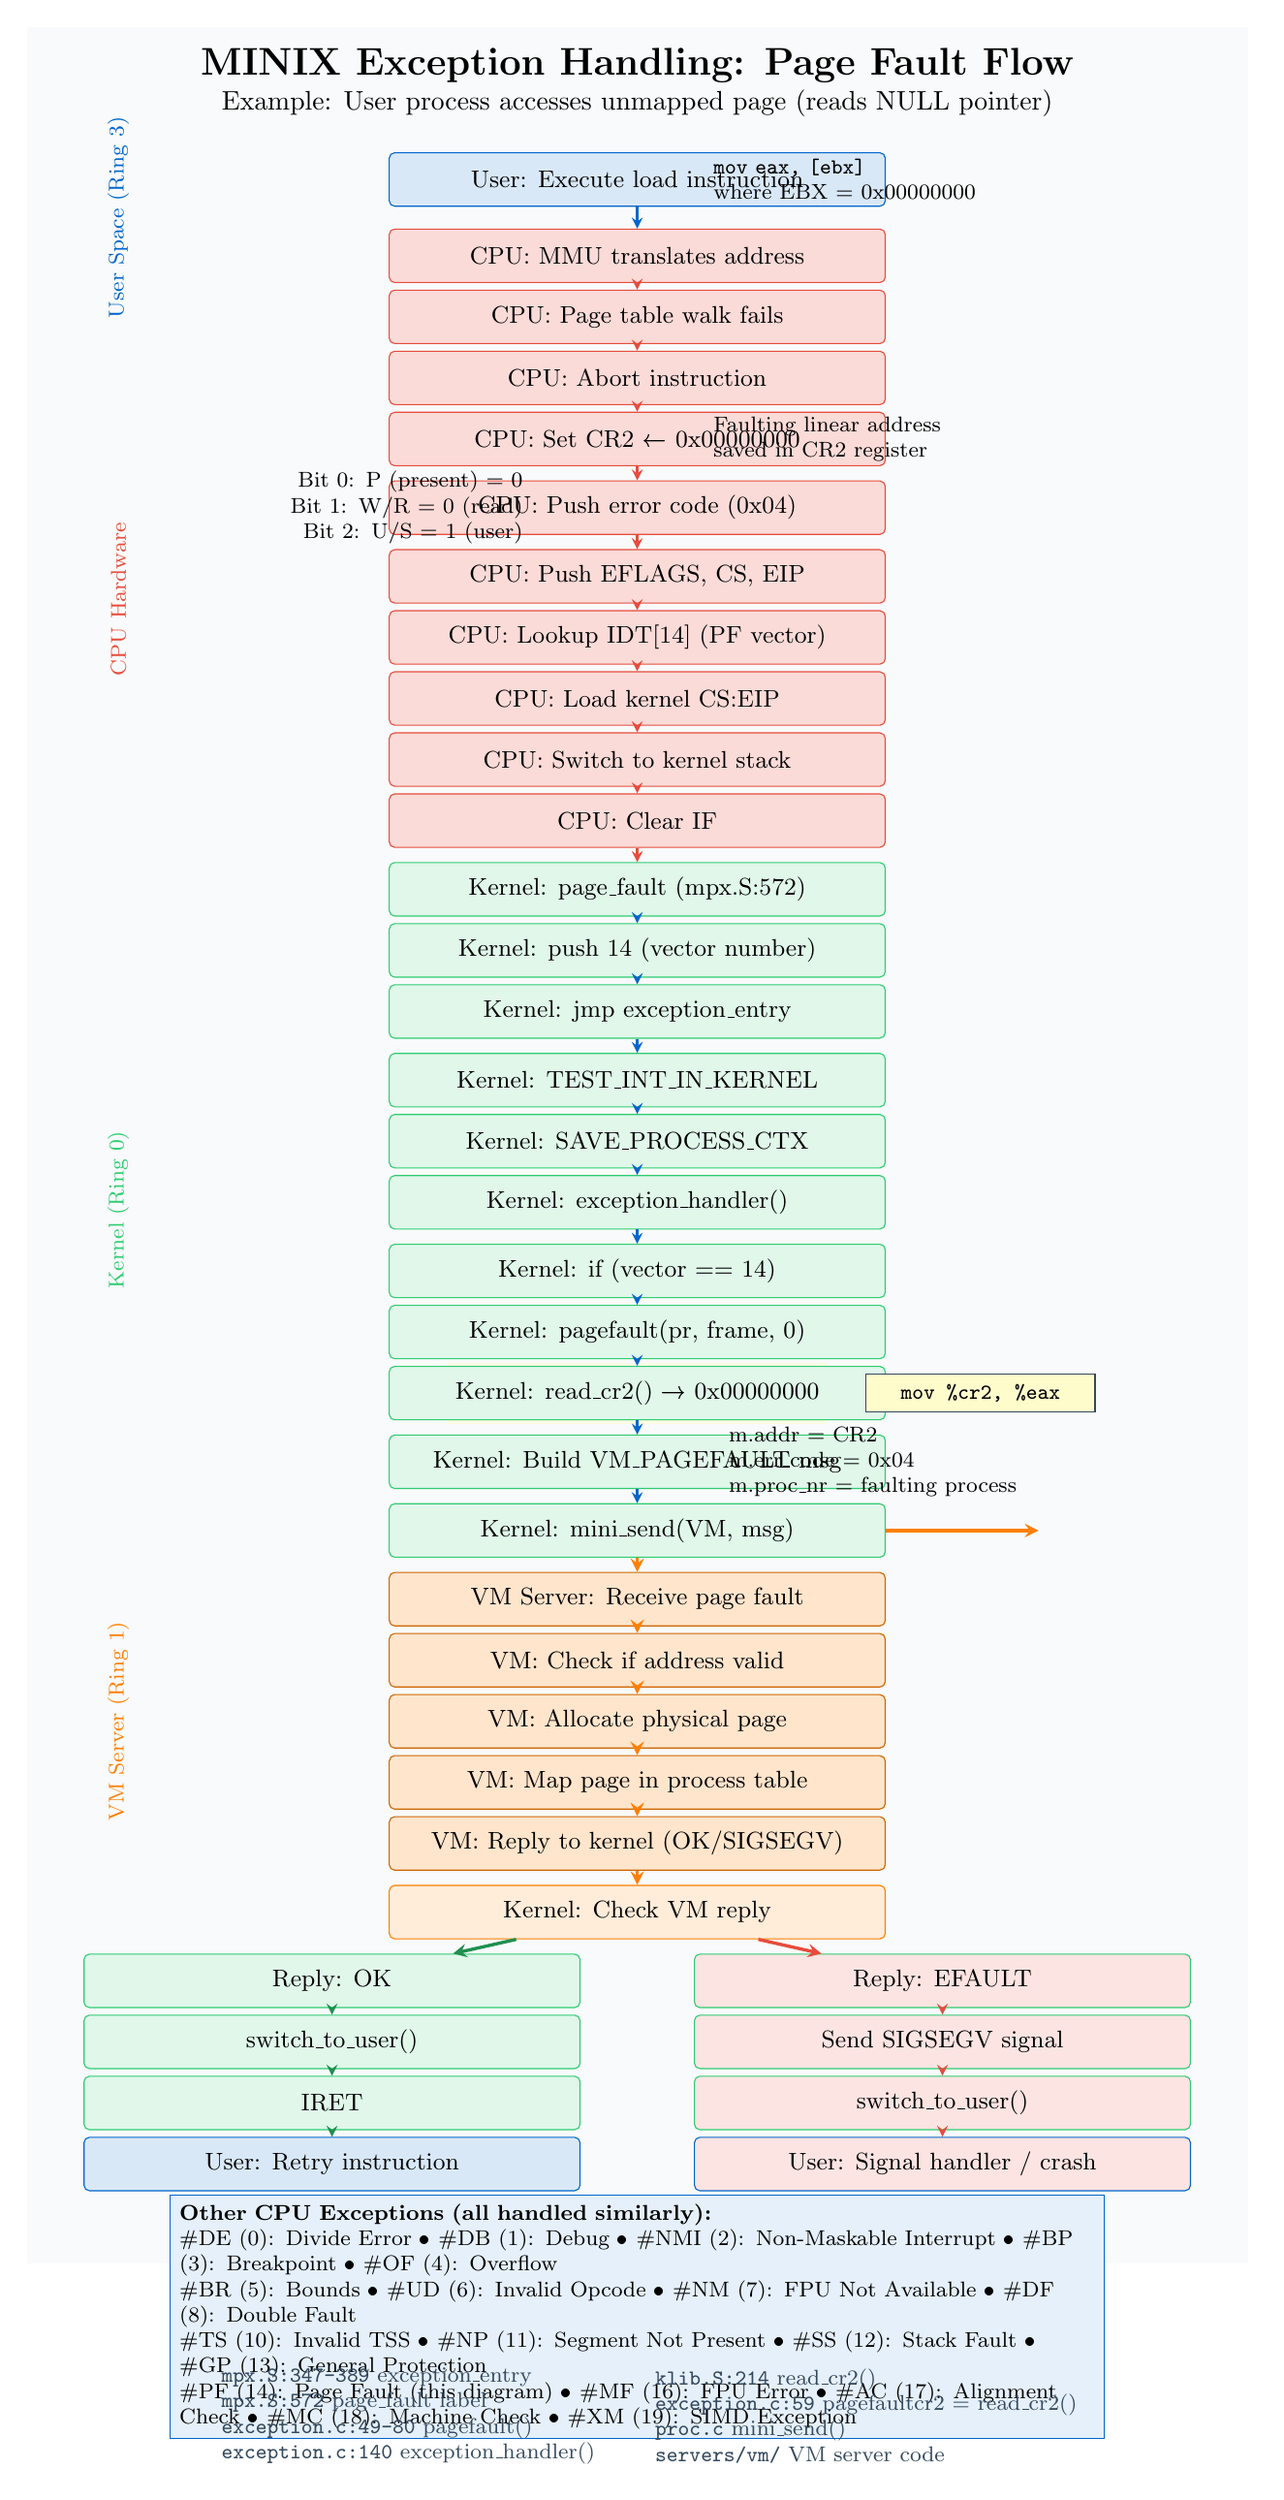
\begin{tikzpicture}[
    box/.style={rectangle, rounded corners=2pt, draw=primaryblue, fill=primaryblue!15, minimum width=6.5cm, minimum height=0.7cm, font=\small, align=center},
    hw/.style={rectangle, rounded corners=2pt, draw=warningred, fill=warningred!20, minimum width=6.5cm, minimum height=0.7cm, font=\small, align=center},
    kernelbox/.style={rectangle, rounded corners=2pt, draw=secondarygreen, fill=secondarygreen!15, minimum width=6.5cm, minimum height=0.7cm, font=\small, align=center},
    server/.style={rectangle, rounded corners=2pt, draw=accentorange!80!black, fill=accentorange!20, minimum width=6.5cm, minimum height=0.7cm, font=\small, align=center},
    arrow/.style={->, >=stealth, thick},
    flow/.style={arrow, primaryblue},
    hwflow/.style={arrow, warningred},
    ipcflow/.style={arrow, accentorange, line width=1.2pt},
    label/.style={font=\footnotesize},
    regbox/.style={rectangle, draw=darkgray, fill=yellow!20, minimum width=3cm, minimum height=0.5cm, font=\footnotesize\ttfamily}
]

% Title
\node[font=\Large\bfseries] at (6, 17) {MINIX Exception Handling: Page Fault Flow};
\node[font=\normalsize] at (6, 16.5) {Example: User process accesses unmapped page (reads NULL pointer)};

% User execution
\node[box] (user1) at (6, 15.5) {User: Execute load instruction};
\node[label, text width=7cm, align=left] at (10.5, 15.5) {
    \texttt{mov eax, [ebx]}\\
    where EBX = 0x00000000
};

% CPU detects fault
\node[hw] (cpu1) at (6, 14.5) {CPU: MMU translates address};
\node[hw] (cpu2) at (6, 13.7) {CPU: Page table walk fails};
\node[hw] (cpu3) at (6, 12.9) {CPU: Abort instruction};
\node[hw] (cpu4) at (6, 12.1) {CPU: Set CR2 ← 0x00000000};
\node[label, text width=6cm, align=left] at (10, 12.1) {
    Faulting linear address\\
    saved in CR2 register
};

% Standard exception entry
\node[hw] (cpu5) at (6, 11.2) {CPU: Push error code (0x04)};
\node[label, text width=5cm, align=right] at (2, 11.2) {
    Bit 0: P (present) = 0\\
    Bit 1: W/R = 0 (read)\\
    Bit 2: U/S = 1 (user)
};
\node[hw] (cpu6) at (6, 10.3) {CPU: Push EFLAGS, CS, EIP};
\node[hw] (cpu7) at (6, 9.5) {CPU: Lookup IDT[14] (PF vector)};
\node[hw] (cpu8) at (6, 8.7) {CPU: Load kernel CS:EIP};
\node[hw] (cpu9) at (6, 7.9) {CPU: Switch to kernel stack};
\node[hw] (cpu10) at (6, 7.1) {CPU: Clear IF};

% Kernel exception entry
\node[kernelbox] (kern1) at (6, 6.2) {Kernel: page\_fault (mpx.S:572)};
\node[kernelbox] (kern2) at (6, 5.4) {Kernel: push 14 (vector number)};
\node[kernelbox] (kern3) at (6, 4.6) {Kernel: jmp exception\_entry};

% Context save
\node[kernelbox] (kern4) at (6, 3.7) {Kernel: TEST\_INT\_IN\_KERNEL};
\node[kernelbox] (kern5) at (6, 2.9) {Kernel: SAVE\_PROCESS\_CTX};
\node[kernelbox] (kern6) at (6, 2.1) {Kernel: exception\_handler()};

% Read CR2
\node[kernelbox] (kern7) at (6, 1.2) {Kernel: if (vector == 14)};
\node[kernelbox] (kern8) at (6, 0.4) {Kernel: pagefault(pr, frame, 0)};
\node[kernelbox] (kern9) at (6, -0.4) {Kernel: read\_cr2() → 0x00000000};
\node[regbox] at (10.5, -0.4) {mov \%cr2, \%eax};

% Build message for VM
\node[kernelbox] (kern10) at (6, -1.3) {Kernel: Build VM\_PAGEFAULT msg};
\node[label, text width=6cm, align=left] at (10.2, -1.3) {
    m.addr = CR2\\
    m.err\_code = 0x04\\
    m.proc\_nr = faulting process
};

% Send IPC to VM
\node[kernelbox] (kern11) at (6, -2.2) {Kernel: mini\_send(VM, msg)};
\node[ipcflow, line width=2pt] (ipc_arrow) at (9.5, -2.2) {};
\draw[ipcflow] (kern11.east) -- ++(2,0);

% VM server handles
\node[server] (vm1) at (6, -3.1) {VM Server: Receive page fault};
\node[server] (vm2) at (6, -3.9) {VM: Check if address valid};
\node[server] (vm3) at (6, -4.7) {VM: Allocate physical page};
\node[server] (vm4) at (6, -5.5) {VM: Map page in process table};
\node[server] (vm5) at (6, -6.3) {VM: Reply to kernel (OK/SIGSEGV)};

% Decision point
\node[kernelbox, fill=accentorange!15, draw=accentorange] (kern12) at (6, -7.2) {Kernel: Check VM reply};

% Two outcomes
\node[kernelbox] (ok1) at (2, -8.1) {Reply: OK};
\node[kernelbox] (ok2) at (2, -8.9) {switch\_to\_user()};
\node[kernelbox] (ok3) at (2, -9.7) {IRET};
\node[box] (ok4) at (2, -10.5) {User: Retry instruction};
\node[label, secondarygreen, font=\bfseries] at (2, -11.2) {Success: Page mapped};

\node[kernelbox, fill=warningred!15] (fail1) at (10, -8.1) {Reply: EFAULT};
\node[kernelbox, fill=warningred!15] (fail2) at (10, -8.9) {Send SIGSEGV signal};
\node[kernelbox, fill=warningred!15] (fail3) at (10, -9.7) {switch\_to\_user()};
\node[box, fill=warningred!15] (fail4) at (10, -10.5) {User: Signal handler / crash};
\node[label, warningred, font=\bfseries] at (10, -11.2) {Failure: Invalid access};

% Flow arrows
\draw[flow] (user1) -- (cpu1);
\draw[hwflow] (cpu1) -- (cpu2);
\draw[hwflow] (cpu2) -- (cpu3);
\draw[hwflow] (cpu3) -- (cpu4);
\draw[hwflow] (cpu4) -- (cpu5);
\draw[hwflow] (cpu5) -- (cpu6);
\draw[hwflow] (cpu6) -- (cpu7);
\draw[hwflow] (cpu7) -- (cpu8);
\draw[hwflow] (cpu8) -- (cpu9);
\draw[hwflow] (cpu9) -- (cpu10);
\draw[hwflow] (cpu10) -- (kern1);
\draw[flow] (kern1) -- (kern2);
\draw[flow] (kern2) -- (kern3);
\draw[flow] (kern3) -- (kern4);
\draw[flow] (kern4) -- (kern5);
\draw[flow] (kern5) -- (kern6);
\draw[flow] (kern6) -- (kern7);
\draw[flow] (kern7) -- (kern8);
\draw[flow] (kern8) -- (kern9);
\draw[flow] (kern9) -- (kern10);
\draw[flow] (kern10) -- (kern11);
\draw[ipcflow] (kern11) -- (vm1);
\draw[ipcflow] (vm1) -- (vm2);
\draw[ipcflow] (vm2) -- (vm3);
\draw[ipcflow] (vm3) -- (vm4);
\draw[ipcflow] (vm4) -- (vm5);
\draw[ipcflow] (vm5) -- (kern12);

\draw[flow, secondarygreen!70!black, line width=1.2pt] (kern12) -- (ok1);
\draw[flow, secondarygreen!70!black] (ok1) -- (ok2);
\draw[flow, secondarygreen!70!black] (ok2) -- (ok3);
\draw[flow, secondarygreen!70!black] (ok3) -- (ok4);

\draw[flow, warningred, line width=1.2pt] (kern12) -- (fail1);
\draw[flow, warningred] (fail1) -- (fail2);
\draw[flow, warningred] (fail2) -- (fail3);
\draw[flow, warningred] (fail3) -- (fail4);

% Background
\begin{scope}[on background layer]
    \fill[lightgray!30] (-2, 17.5) rectangle (14, -11.8);
    % Highlight CR2 read
    \fill[yellow!20, opacity=0.5] (3.5, -0.8) rectangle (8.5, 0);
\end{scope}

% Side annotations
\node[font=\footnotesize, rotate=90, primaryblue] at (-0.8, 15) {User Space (Ring 3)};
\node[font=\footnotesize, rotate=90, warningred] at (-0.8, 10) {CPU Hardware};
\node[font=\footnotesize, rotate=90, secondarygreen] at (-0.8, 2) {Kernel (Ring 0)};
\node[font=\footnotesize, rotate=90, accentorange] at (-0.8, -4.7) {VM Server (Ring 1)};

% Exception types reference
\node[rectangle, draw=primaryblue, fill=primaryblue!10, text width=12cm, align=left, font=\footnotesize] at (6, -12.5) {
\textbf{Other CPU Exceptions (all handled similarly):}\\
\#DE (0): Divide Error • \#DB (1): Debug • \#NMI (2): Non-Maskable Interrupt • \#BP (3): Breakpoint • \#OF (4): Overflow\\
\#BR (5): Bounds • \#UD (6): Invalid Opcode • \#NM (7): FPU Not Available • \#DF (8): Double Fault\\
\#TS (10): Invalid TSS • \#NP (11): Segment Not Present • \#SS (12): Stack Fault • \#GP (13): General Protection\\
\#PF (14): Page Fault (this diagram) • \#MF (16): FPU Error • \#AC (17): Alignment Check • \#MC (18): Machine Check • \#XM (19): SIMD Exception
};

% File references
\node[font=\footnotesize, text=darkgray, align=left] at (3, -13.8) {
\texttt{mpx.S:347-389} exception\_entry\\
\texttt{mpx.S:572} page\_fault label\\
\texttt{exception.c:49-80} pagefault()\\
\texttt{exception.c:140} exception\_handler()
};

\node[font=\footnotesize, text=darkgray, align=left] at (9, -13.8) {
\texttt{klib.S:214} read\_cr2()\\
\texttt{exception.c:59} pagefaultcr2 = read\_cr2()\\
\texttt{proc.c} mini\_send()\\
\texttt{servers/vm/} VM server code
};

\end{tikzpicture}
\end{document}
